\documentclass[twoside]{book}

% Packages required by doxygen
\usepackage{calc}
\usepackage{doxygen}
\usepackage{graphicx}
\usepackage[utf8]{inputenc}
\usepackage{makeidx}
\usepackage{multicol}
\usepackage{multirow}
\usepackage{textcomp}
\usepackage[table]{xcolor}

% Font selection
\usepackage[T1]{fontenc}
\usepackage{mathptmx}
\usepackage[scaled=.90]{helvet}
\usepackage{courier}
\usepackage{amssymb}
\usepackage{sectsty}
\renewcommand{\familydefault}{\sfdefault}
\allsectionsfont{%
  \fontseries{bc}\selectfont%
  \color{darkgray}%
}
\renewcommand{\DoxyLabelFont}{%
  \fontseries{bc}\selectfont%
  \color{darkgray}%
}

% Page & text layout
\usepackage{geometry}
\geometry{%
  a4paper,%
  top=2.5cm,%
  bottom=2.5cm,%
  left=2.5cm,%
  right=2.5cm%
}
\tolerance=750
\hfuzz=15pt
\hbadness=750
\setlength{\emergencystretch}{15pt}
\setlength{\parindent}{0cm}
\setlength{\parskip}{0.2cm}
\makeatletter
\renewcommand{\paragraph}{%
  \@startsection{paragraph}{4}{0ex}{-1.0ex}{1.0ex}{%
    \normalfont\normalsize\bfseries\SS@parafont%
  }%
}
\renewcommand{\subparagraph}{%
  \@startsection{subparagraph}{5}{0ex}{-1.0ex}{1.0ex}{%
    \normalfont\normalsize\bfseries\SS@subparafont%
  }%
}
\makeatother

% Headers & footers
\usepackage{fancyhdr}
\pagestyle{fancyplain}
\fancyhead[LE]{\fancyplain{}{\bfseries\thepage}}
\fancyhead[CE]{\fancyplain{}{}}
\fancyhead[RE]{\fancyplain{}{\bfseries\leftmark}}
\fancyhead[LO]{\fancyplain{}{\bfseries\rightmark}}
\fancyhead[CO]{\fancyplain{}{}}
\fancyhead[RO]{\fancyplain{}{\bfseries\thepage}}
\fancyfoot[LE]{\fancyplain{}{}}
\fancyfoot[CE]{\fancyplain{}{}}
\fancyfoot[RE]{\fancyplain{}{\bfseries\scriptsize Generated on Sat Jan 25 2014 21\-:57\-:31 for I\-H\-M\-\_\-\-O\-F\-E\-L\-I by Doxygen }}
\fancyfoot[LO]{\fancyplain{}{\bfseries\scriptsize Generated on Sat Jan 25 2014 21\-:57\-:31 for I\-H\-M\-\_\-\-O\-F\-E\-L\-I by Doxygen }}
\fancyfoot[CO]{\fancyplain{}{}}
\fancyfoot[RO]{\fancyplain{}{}}
\renewcommand{\footrulewidth}{0.4pt}
\renewcommand{\chaptermark}[1]{%
  \markboth{#1}{}%
}
\renewcommand{\sectionmark}[1]{%
  \markright{\thesection\ #1}%
}

% Indices & bibliography
\usepackage{natbib}
\usepackage[titles]{tocloft}
\setcounter{tocdepth}{3}
\setcounter{secnumdepth}{5}
\makeindex

% Hyperlinks (required, but should be loaded last)
\usepackage{ifpdf}
\ifpdf
  \usepackage[pdftex,pagebackref=true]{hyperref}
\else
  \usepackage[ps2pdf,pagebackref=true]{hyperref}
\fi
\hypersetup{%
  colorlinks=true,%
  linkcolor=blue,%
  citecolor=blue,%
  unicode%
}

% Custom commands
\newcommand{\clearemptydoublepage}{%
  \newpage{\pagestyle{empty}\cleardoublepage}%
}


%===== C O N T E N T S =====

\begin{document}

% Titlepage & ToC
\hypersetup{pageanchor=false}
\pagenumbering{roman}
\begin{titlepage}
\vspace*{7cm}
\begin{center}%
{\Large I\-H\-M\-\_\-\-O\-F\-E\-L\-I }\\
\vspace*{1cm}
{\large Generated by Doxygen 1.8.6}\\
\vspace*{0.5cm}
{\small Sat Jan 25 2014 21:57:31}\\
\end{center}
\end{titlepage}
\clearemptydoublepage
\tableofcontents
\clearemptydoublepage
\pagenumbering{arabic}
\hypersetup{pageanchor=true}

%--- Begin generated contents ---
\chapter{I\-H\-M\-\_\-\-O\-F\-E\-L\-I}
\label{md_README}
\hypertarget{md_README}{}
This program has been created to modify the data files used with O\-F\-E\-L\-I. Those files are written in X\-M\-L and have the extension \char`\"{}.\-dat\char`\"{}. The only requirement to use it is to install Qt (follow this link for more information \href{http://qt-project.org/doc/qt-4.8/installation.html}{\tt Installation Qt}

To build the program from sources you can use the script \char`\"{}compil\char`\"{}, or you can follow this procedure \-:
\begin{DoxyItemize}
\item launch the command \char`\"{}qmake -\/o Makefile I\-H\-M\-\_\-\-O\-F\-E\-L\-I.\-pro\char`\"{} to generate the makefile
\item then use \char`\"{}make\char`\"{} to build the program, this will create an executable named I\-H\-M\-\_\-\-O\-F\-E\-L\-I To launch the program, just use \char`\"{}./\-I\-H\-M\-\_\-\-O\-F\-E\-L\-I\char`\"{}.
\end{DoxyItemize}

With this program you can create a new data file for O\-F\-E\-L\-I or modify an existing file. The creation of a new file can be performed by using the default file provided with the program as a base. Once this file is opened, you can modify it as you wish. For the modification, this program allows you to perform all the operations you should need (add/delete tag, add/delete comment, modification of a tag, modification of attributes). 
\chapter{Hierarchical Index}
\section{Class Hierarchy}
This inheritance list is sorted roughly, but not completely, alphabetically\-:\begin{DoxyCompactList}
\item Q\-Dialog\begin{DoxyCompactList}
\item \contentsline{section}{Dialog\-About}{\pageref{classDialogAbout}}{}
\item \contentsline{section}{Dialog\-Add\-Comment}{\pageref{classDialogAddComment}}{}
\item \contentsline{section}{Dialog\-Add\-Node}{\pageref{classDialogAddNode}}{}
\item \contentsline{section}{Dialog\-Exec}{\pageref{classDialogExec}}{}
\item \contentsline{section}{Dialog\-Modify\-Node}{\pageref{classDialogModifyNode}}{}
\item \contentsline{section}{Dialog\-Save}{\pageref{classDialogSave}}{}
\end{DoxyCompactList}
\item Q\-Main\-Window\begin{DoxyCompactList}
\item \contentsline{section}{Main\-Window}{\pageref{classMainWindow}}{}
\end{DoxyCompactList}
\end{DoxyCompactList}

\chapter{Class Index}
\section{Class List}
Here are the classes, structs, unions and interfaces with brief descriptions\-:\begin{DoxyCompactList}
\item\contentsline{section}{\hyperlink{classDialogAddComment}{Dialog\-Add\-Comment} \\*Manages the addition of a comment }{\pageref{classDialogAddComment}}{}
\item\contentsline{section}{\hyperlink{classDialogAddNode}{Dialog\-Add\-Node} \\*Manages the addition of a node }{\pageref{classDialogAddNode}}{}
\item\contentsline{section}{\hyperlink{classDialogExec}{Dialog\-Exec} \\*Manages the execution of the O\-F\-E\-L\-I program }{\pageref{classDialogExec}}{}
\item\contentsline{section}{\hyperlink{classDialogModifyNode}{Dialog\-Modify\-Node} \\*Manages the modification of a node in the Tree\-View }{\pageref{classDialogModifyNode}}{}
\item\contentsline{section}{\hyperlink{classDialogSave}{Dialog\-Save} \\*Manages the dialog shown when the user close the program but didn't save his file }{\pageref{classDialogSave}}{}
\item\contentsline{section}{\hyperlink{classMainWindow}{Main\-Window} \\*Manages all the user interface }{\pageref{classMainWindow}}{}
\end{DoxyCompactList}

\chapter{Class Documentation}
\hypertarget{classDialogAddComment}{\section{Dialog\-Add\-Comment Class Reference}
\label{classDialogAddComment}\index{Dialog\-Add\-Comment@{Dialog\-Add\-Comment}}
}


The \hyperlink{classDialogAddComment}{Dialog\-Add\-Comment} class manages the addition of a comment.  




{\ttfamily \#include $<$dialogaddcomment.\-h$>$}

Inheritance diagram for Dialog\-Add\-Comment\-:\begin{figure}[H]
\begin{center}
\leavevmode
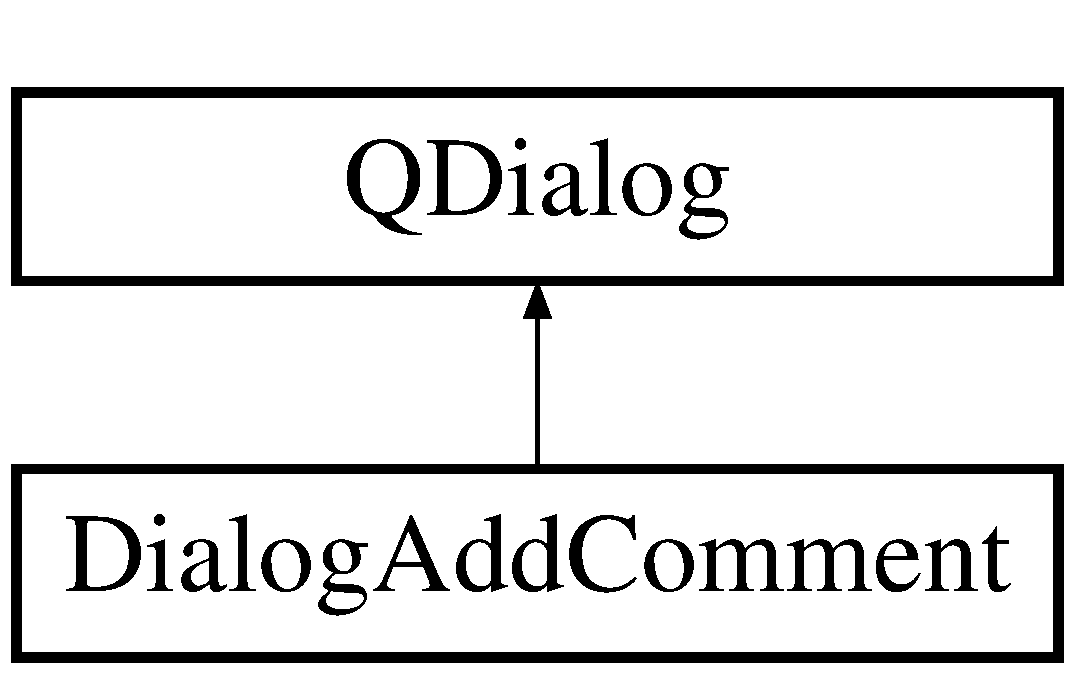
\includegraphics[height=2.000000cm]{classDialogAddComment}
\end{center}
\end{figure}
\subsection*{Public Slots}
\begin{DoxyCompactItemize}
\item 
\hypertarget{classDialogAddComment_a78aac814a6aa24e09b45730b601a99db}{void \hyperlink{classDialogAddComment_a78aac814a6aa24e09b45730b601a99db}{add\-Comment} ()}\label{classDialogAddComment_a78aac814a6aa24e09b45730b601a99db}

\begin{DoxyCompactList}\small\item\em Add the comment to the Tree\-View (and to the document) by calling tha add\-Comment function of the \hyperlink{classMainWindow}{Main\-Window}. \end{DoxyCompactList}\end{DoxyCompactItemize}
\subsection*{Public Member Functions}
\begin{DoxyCompactItemize}
\item 
\hyperlink{classDialogAddComment_ad0cdceadc62c07e6fba1e0a2f2ab71eb}{Dialog\-Add\-Comment} (Q\-String parent\-Node, int selected\-Row, \hyperlink{classMainWindow}{Main\-Window} $\ast$parent=0)
\begin{DoxyCompactList}\small\item\em \hyperlink{classDialogAddComment}{Dialog\-Add\-Comment}. \end{DoxyCompactList}\end{DoxyCompactItemize}
\subsection*{Private Attributes}
\begin{DoxyCompactItemize}
\item 
\hypertarget{classDialogAddComment_afc346797c1b728c2dd1acd01414e7c04}{Ui\-::\-Dialog\-Add\-Comment $\ast$ {\bfseries ui}}\label{classDialogAddComment_afc346797c1b728c2dd1acd01414e7c04}

\item 
\hypertarget{classDialogAddComment_aaed388d10eaecfe0bae9c623485d723c}{Q\-String {\bfseries parent\-Node}}\label{classDialogAddComment_aaed388d10eaecfe0bae9c623485d723c}

\item 
\hypertarget{classDialogAddComment_a600ac817234534656aefda60006f6f67}{int {\bfseries selected\-Row}}\label{classDialogAddComment_a600ac817234534656aefda60006f6f67}

\item 
\hypertarget{classDialogAddComment_a239dfaac007faeab5f04f7a36177f1ac}{\hyperlink{classMainWindow}{Main\-Window} $\ast$ {\bfseries parent}}\label{classDialogAddComment_a239dfaac007faeab5f04f7a36177f1ac}

\end{DoxyCompactItemize}


\subsection{Detailed Description}
The \hyperlink{classDialogAddComment}{Dialog\-Add\-Comment} class manages the addition of a comment. 

\subsection{Constructor \& Destructor Documentation}
\hypertarget{classDialogAddComment_ad0cdceadc62c07e6fba1e0a2f2ab71eb}{\index{Dialog\-Add\-Comment@{Dialog\-Add\-Comment}!Dialog\-Add\-Comment@{Dialog\-Add\-Comment}}
\index{Dialog\-Add\-Comment@{Dialog\-Add\-Comment}!DialogAddComment@{Dialog\-Add\-Comment}}
\subsubsection[{Dialog\-Add\-Comment}]{\setlength{\rightskip}{0pt plus 5cm}Dialog\-Add\-Comment\-::\-Dialog\-Add\-Comment (
\begin{DoxyParamCaption}
\item[{Q\-String}]{parent\-Node, }
\item[{int}]{selected\-Row, }
\item[{{\bf Main\-Window} $\ast$}]{parent = {\ttfamily 0}}
\end{DoxyParamCaption}
)\hspace{0.3cm}{\ttfamily [explicit]}}}\label{classDialogAddComment_ad0cdceadc62c07e6fba1e0a2f2ab71eb}


\hyperlink{classDialogAddComment}{Dialog\-Add\-Comment}. 


\begin{DoxyParams}{Parameters}
{\em parent\-Node} & The name of the parent node \\
\hline
{\em selected\-Row} & The row number of the selected node \\
\hline
{\em parent} & \\
\hline
\end{DoxyParams}


The documentation for this class was generated from the following files\-:\begin{DoxyCompactItemize}
\item 
dialogaddcomment.\-h\item 
dialogaddcomment.\-cpp\end{DoxyCompactItemize}

\hypertarget{classDialogAddNode}{\section{Dialog\-Add\-Node Class Reference}
\label{classDialogAddNode}\index{Dialog\-Add\-Node@{Dialog\-Add\-Node}}
}


The \hyperlink{classDialogAddNode}{Dialog\-Add\-Node} class manages the addition of a node.  




{\ttfamily \#include $<$dialogaddnode.\-h$>$}

Inheritance diagram for Dialog\-Add\-Node\-:\begin{figure}[H]
\begin{center}
\leavevmode
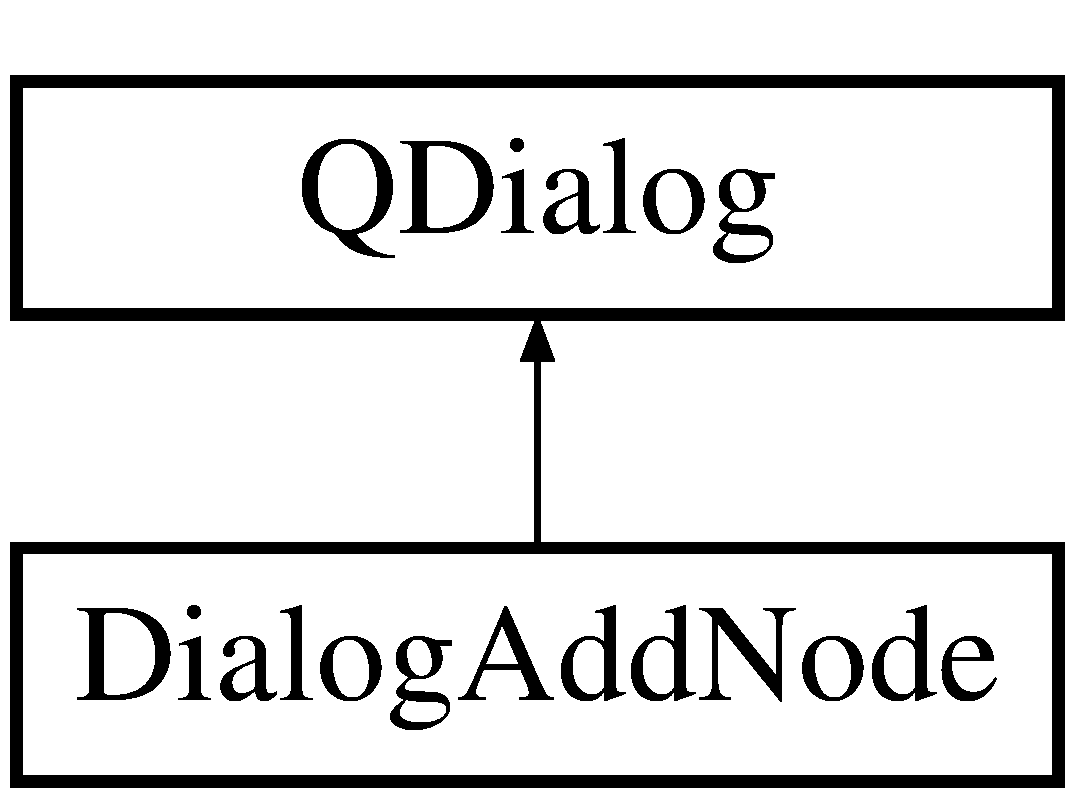
\includegraphics[height=2.000000cm]{classDialogAddNode}
\end{center}
\end{figure}
\subsection*{Public Slots}
\begin{DoxyCompactItemize}
\item 
\hypertarget{classDialogAddNode_a2335a5fef409594fd2e73330870b12c6}{void \hyperlink{classDialogAddNode_a2335a5fef409594fd2e73330870b12c6}{add\-Node} ()}\label{classDialogAddNode_a2335a5fef409594fd2e73330870b12c6}

\begin{DoxyCompactList}\small\item\em Add the node to the Tree\-View (and to the document) by calling tha add\-Node function of the \hyperlink{classMainWindow}{Main\-Window}. \end{DoxyCompactList}\end{DoxyCompactItemize}
\subsection*{Public Member Functions}
\begin{DoxyCompactItemize}
\item 
\hyperlink{classDialogAddNode_a9f573b099436b835e4c660e81e361f75}{Dialog\-Add\-Node} (Q\-String\-List $\ast$parent\-List, \hyperlink{classMainWindow}{Main\-Window} $\ast$parent)
\begin{DoxyCompactList}\small\item\em Constructor. \end{DoxyCompactList}\end{DoxyCompactItemize}
\subsection*{Private Attributes}
\begin{DoxyCompactItemize}
\item 
\hypertarget{classDialogAddNode_a1b64236defb36192a04a69e706d9e62d}{Ui\-::\-Dialog\-Add\-Node $\ast$ {\bfseries ui}}\label{classDialogAddNode_a1b64236defb36192a04a69e706d9e62d}

\item 
\hypertarget{classDialogAddNode_ad5002ef98ac93a838d5ed883f3a969ac}{Q\-String\-List $\ast$ {\bfseries node\-Name\-List}}\label{classDialogAddNode_ad5002ef98ac93a838d5ed883f3a969ac}

\item 
\hypertarget{classDialogAddNode_a1ccc4570ab17afc7cff38f7eaa4bd752}{\hyperlink{classMainWindow}{Main\-Window} $\ast$ {\bfseries parent}}\label{classDialogAddNode_a1ccc4570ab17afc7cff38f7eaa4bd752}

\end{DoxyCompactItemize}


\subsection{Detailed Description}
The \hyperlink{classDialogAddNode}{Dialog\-Add\-Node} class manages the addition of a node. 

\subsection{Constructor \& Destructor Documentation}
\hypertarget{classDialogAddNode_a9f573b099436b835e4c660e81e361f75}{\index{Dialog\-Add\-Node@{Dialog\-Add\-Node}!Dialog\-Add\-Node@{Dialog\-Add\-Node}}
\index{Dialog\-Add\-Node@{Dialog\-Add\-Node}!DialogAddNode@{Dialog\-Add\-Node}}
\subsubsection[{Dialog\-Add\-Node}]{\setlength{\rightskip}{0pt plus 5cm}Dialog\-Add\-Node\-::\-Dialog\-Add\-Node (
\begin{DoxyParamCaption}
\item[{Q\-String\-List $\ast$}]{parent\-List, }
\item[{{\bf Main\-Window} $\ast$}]{parent}
\end{DoxyParamCaption}
)\hspace{0.3cm}{\ttfamily [explicit]}}}\label{classDialogAddNode_a9f573b099436b835e4c660e81e361f75}


Constructor. 


\begin{DoxyParams}{Parameters}
{\em parent\-List} & The list of possibles parent to the new node. \\
\hline
{\em parent} & \\
\hline
\end{DoxyParams}


The documentation for this class was generated from the following files\-:\begin{DoxyCompactItemize}
\item 
dialogaddnode.\-h\item 
dialogaddnode.\-cpp\end{DoxyCompactItemize}

\hypertarget{classDialogExec}{\section{Dialog\-Exec Class Reference}
\label{classDialogExec}\index{Dialog\-Exec@{Dialog\-Exec}}
}


The \hyperlink{classDialogExec}{Dialog\-Exec} class manages the execution of the O\-F\-E\-L\-I program.  




{\ttfamily \#include $<$dialogexec.\-h$>$}

Inheritance diagram for Dialog\-Exec\-:\begin{figure}[H]
\begin{center}
\leavevmode
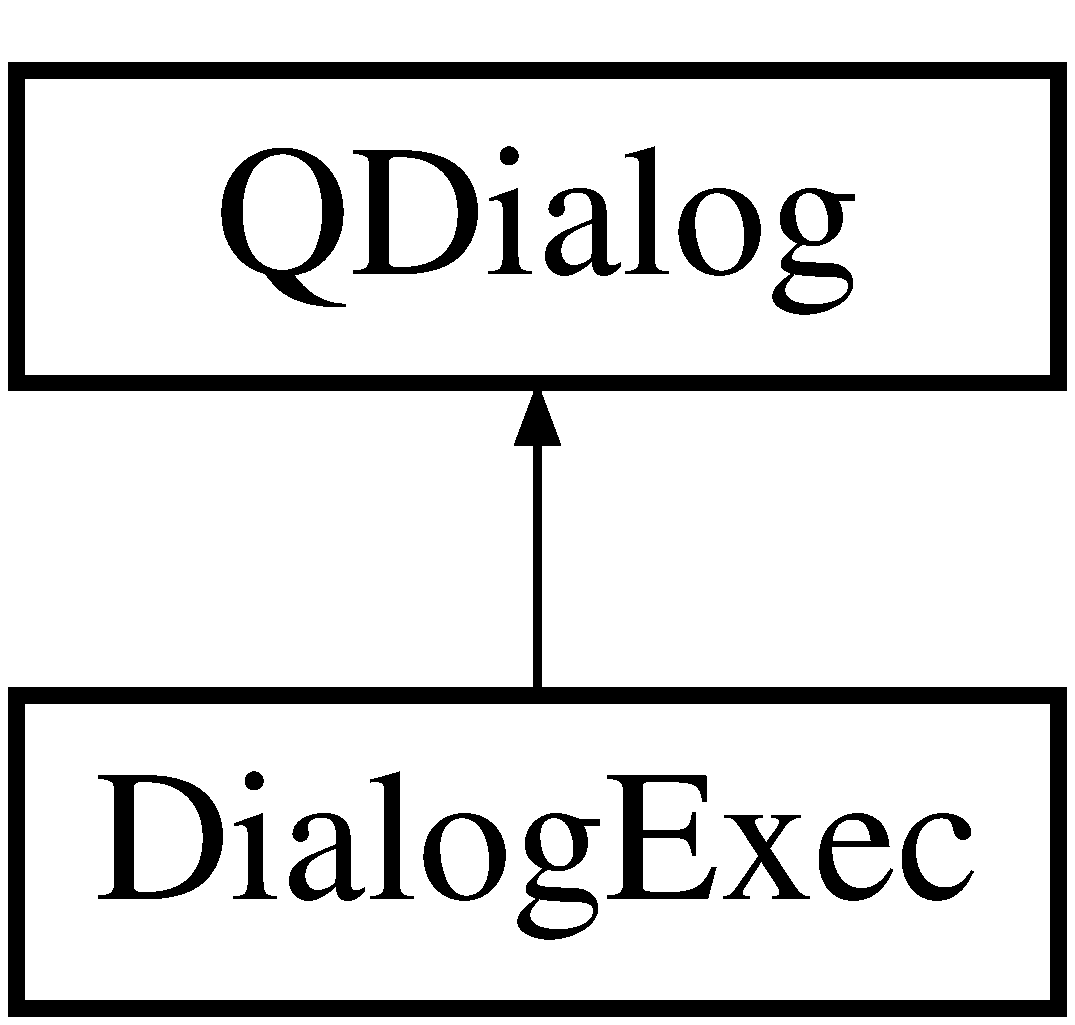
\includegraphics[height=2.000000cm]{classDialogExec}
\end{center}
\end{figure}
\subsection*{Public Slots}
\begin{DoxyCompactItemize}
\item 
\hypertarget{classDialogExec_ab33c3a148cfaa7d2969b9c42b4f97911}{void \hyperlink{classDialogExec_ab33c3a148cfaa7d2969b9c42b4f97911}{select\-Exec} ()}\label{classDialogExec_ab33c3a148cfaa7d2969b9c42b4f97911}

\begin{DoxyCompactList}\small\item\em Opens a dialog to select the executable for the O\-F\-E\-L\-I program. \end{DoxyCompactList}\item 
\hypertarget{classDialogExec_a8368adc07cebb25e0d78c137ee6149e9}{void \hyperlink{classDialogExec_a8368adc07cebb25e0d78c137ee6149e9}{select\-Dat} ()}\label{classDialogExec_a8368adc07cebb25e0d78c137ee6149e9}

\begin{DoxyCompactList}\small\item\em Opens a dialog to select the data file for the O\-F\-E\-L\-I program. \end{DoxyCompactList}\item 
\hypertarget{classDialogExec_a0911fce2350ffef1f3b72cabf1ca7796}{void \hyperlink{classDialogExec_a0911fce2350ffef1f3b72cabf1ca7796}{execute} ()}\label{classDialogExec_a0911fce2350ffef1f3b72cabf1ca7796}

\begin{DoxyCompactList}\small\item\em Executes the O\-F\-E\-L\-I program and show the result in the \hyperlink{classMainWindow}{Main\-Window}. \end{DoxyCompactList}\end{DoxyCompactItemize}
\subsection*{Public Member Functions}
\begin{DoxyCompactItemize}
\item 
\hyperlink{classDialogExec_a9f886767450f6b4928186051b3b7273b}{Dialog\-Exec} (Q\-Text\-Edit $\ast$parent=0, Q\-String filename\-Dat=\char`\"{}\char`\"{})
\begin{DoxyCompactList}\small\item\em Constructor. \end{DoxyCompactList}\end{DoxyCompactItemize}
\subsection*{Private Attributes}
\begin{DoxyCompactItemize}
\item 
\hypertarget{classDialogExec_af7accc642459f93dcdf365729a9457a2}{Ui\-::\-Dialog\-Exec $\ast$ {\bfseries ui}}\label{classDialogExec_af7accc642459f93dcdf365729a9457a2}

\item 
\hypertarget{classDialogExec_aa6f355f348dcac19a8e4126c6c396c6e}{Q\-Text\-Edit $\ast$ {\bfseries parent}}\label{classDialogExec_aa6f355f348dcac19a8e4126c6c396c6e}

\end{DoxyCompactItemize}


\subsection{Detailed Description}
The \hyperlink{classDialogExec}{Dialog\-Exec} class manages the execution of the O\-F\-E\-L\-I program. 

\subsection{Constructor \& Destructor Documentation}
\hypertarget{classDialogExec_a9f886767450f6b4928186051b3b7273b}{\index{Dialog\-Exec@{Dialog\-Exec}!Dialog\-Exec@{Dialog\-Exec}}
\index{Dialog\-Exec@{Dialog\-Exec}!DialogExec@{Dialog\-Exec}}
\subsubsection[{Dialog\-Exec}]{\setlength{\rightskip}{0pt plus 5cm}Dialog\-Exec\-::\-Dialog\-Exec (
\begin{DoxyParamCaption}
\item[{Q\-Text\-Edit $\ast$}]{parent = {\ttfamily 0}, }
\item[{Q\-String}]{filename\-Dat = {\ttfamily \char`\"{}\char`\"{}}}
\end{DoxyParamCaption}
)\hspace{0.3cm}{\ttfamily [explicit]}}}\label{classDialogExec_a9f886767450f6b4928186051b3b7273b}


Constructor. 


\begin{DoxyParams}{Parameters}
{\em parent} & \\
\hline
{\em filename\-Dat} & The path to the data file \\
\hline
\end{DoxyParams}


The documentation for this class was generated from the following files\-:\begin{DoxyCompactItemize}
\item 
dialogexec.\-h\item 
dialogexec.\-cpp\end{DoxyCompactItemize}

\hypertarget{classDialogModifyNode}{\section{Dialog\-Modify\-Node Class Reference}
\label{classDialogModifyNode}\index{Dialog\-Modify\-Node@{Dialog\-Modify\-Node}}
}


The \hyperlink{classDialogModifyNode}{Dialog\-Modify\-Node} class manages the modification of a node in the Tree\-View.  




{\ttfamily \#include $<$dialogmodifynode.\-h$>$}

Inheritance diagram for Dialog\-Modify\-Node\-:\begin{figure}[H]
\begin{center}
\leavevmode
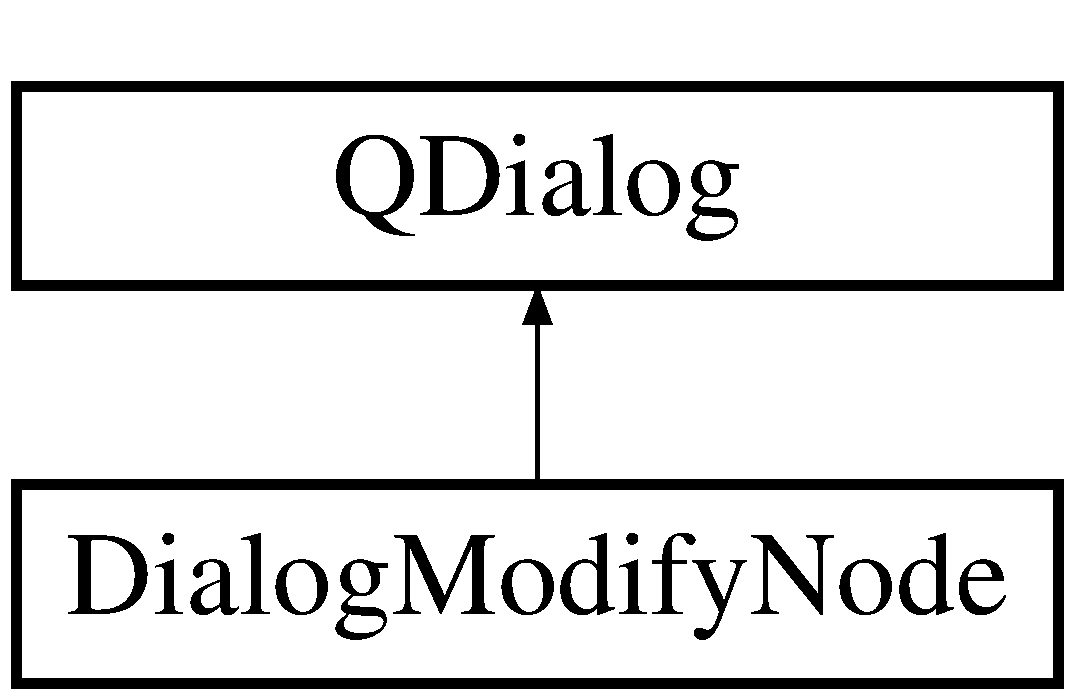
\includegraphics[height=2.000000cm]{classDialogModifyNode}
\end{center}
\end{figure}
\subsection*{Public Slots}
\begin{DoxyCompactItemize}
\item 
\hypertarget{classDialogModifyNode_a93522938fb36db6cca68f92b8360a3ca}{void \hyperlink{classDialogModifyNode_a93522938fb36db6cca68f92b8360a3ca}{modify\-Node} ()}\label{classDialogModifyNode_a93522938fb36db6cca68f92b8360a3ca}

\begin{DoxyCompactList}\small\item\em Modifes the node selected with the new name. \end{DoxyCompactList}\end{DoxyCompactItemize}
\subsection*{Public Member Functions}
\begin{DoxyCompactItemize}
\item 
\hyperlink{classDialogModifyNode_acd9fdede53fb8c97f5fa7ad1984d743f}{Dialog\-Modify\-Node} (\hyperlink{classMainWindow}{Main\-Window} $\ast$parent, Q\-String selected\-Node)
\begin{DoxyCompactList}\small\item\em Constructor. \end{DoxyCompactList}\end{DoxyCompactItemize}
\subsection*{Private Attributes}
\begin{DoxyCompactItemize}
\item 
\hypertarget{classDialogModifyNode_a3c6da5931f73ea1956d16d2ed6119964}{Ui\-::\-Dialog\-Modify\-Node $\ast$ {\bfseries ui}}\label{classDialogModifyNode_a3c6da5931f73ea1956d16d2ed6119964}

\item 
\hypertarget{classDialogModifyNode_a6ee06f908415fe1fb862c976c44a55d1}{\hyperlink{classMainWindow}{Main\-Window} $\ast$ {\bfseries parent}}\label{classDialogModifyNode_a6ee06f908415fe1fb862c976c44a55d1}

\item 
\hypertarget{classDialogModifyNode_a1cb348e6717e76813026a726d5a78baa}{Q\-String {\bfseries selected\-Node}}\label{classDialogModifyNode_a1cb348e6717e76813026a726d5a78baa}

\end{DoxyCompactItemize}


\subsection{Detailed Description}
The \hyperlink{classDialogModifyNode}{Dialog\-Modify\-Node} class manages the modification of a node in the Tree\-View. 

\subsection{Constructor \& Destructor Documentation}
\hypertarget{classDialogModifyNode_acd9fdede53fb8c97f5fa7ad1984d743f}{\index{Dialog\-Modify\-Node@{Dialog\-Modify\-Node}!Dialog\-Modify\-Node@{Dialog\-Modify\-Node}}
\index{Dialog\-Modify\-Node@{Dialog\-Modify\-Node}!DialogModifyNode@{Dialog\-Modify\-Node}}
\subsubsection[{Dialog\-Modify\-Node}]{\setlength{\rightskip}{0pt plus 5cm}Dialog\-Modify\-Node\-::\-Dialog\-Modify\-Node (
\begin{DoxyParamCaption}
\item[{{\bf Main\-Window} $\ast$}]{parent, }
\item[{Q\-String}]{selected\-Node}
\end{DoxyParamCaption}
)\hspace{0.3cm}{\ttfamily [explicit]}}}\label{classDialogModifyNode_acd9fdede53fb8c97f5fa7ad1984d743f}


Constructor. 


\begin{DoxyParams}{Parameters}
{\em parent} & \\
\hline
{\em selected\-Node} & The name of the selected node \\
\hline
\end{DoxyParams}


The documentation for this class was generated from the following files\-:\begin{DoxyCompactItemize}
\item 
dialogmodifynode.\-h\item 
dialogmodifynode.\-cpp\end{DoxyCompactItemize}

\hypertarget{classDialogSave}{\section{Dialog\-Save Class Reference}
\label{classDialogSave}\index{Dialog\-Save@{Dialog\-Save}}
}


The \hyperlink{classDialogSave}{Dialog\-Save} class manages the dialog shown when the user close the program but didn't save his file.  




{\ttfamily \#include $<$dialogsave.\-h$>$}

Inheritance diagram for Dialog\-Save\-:\begin{figure}[H]
\begin{center}
\leavevmode
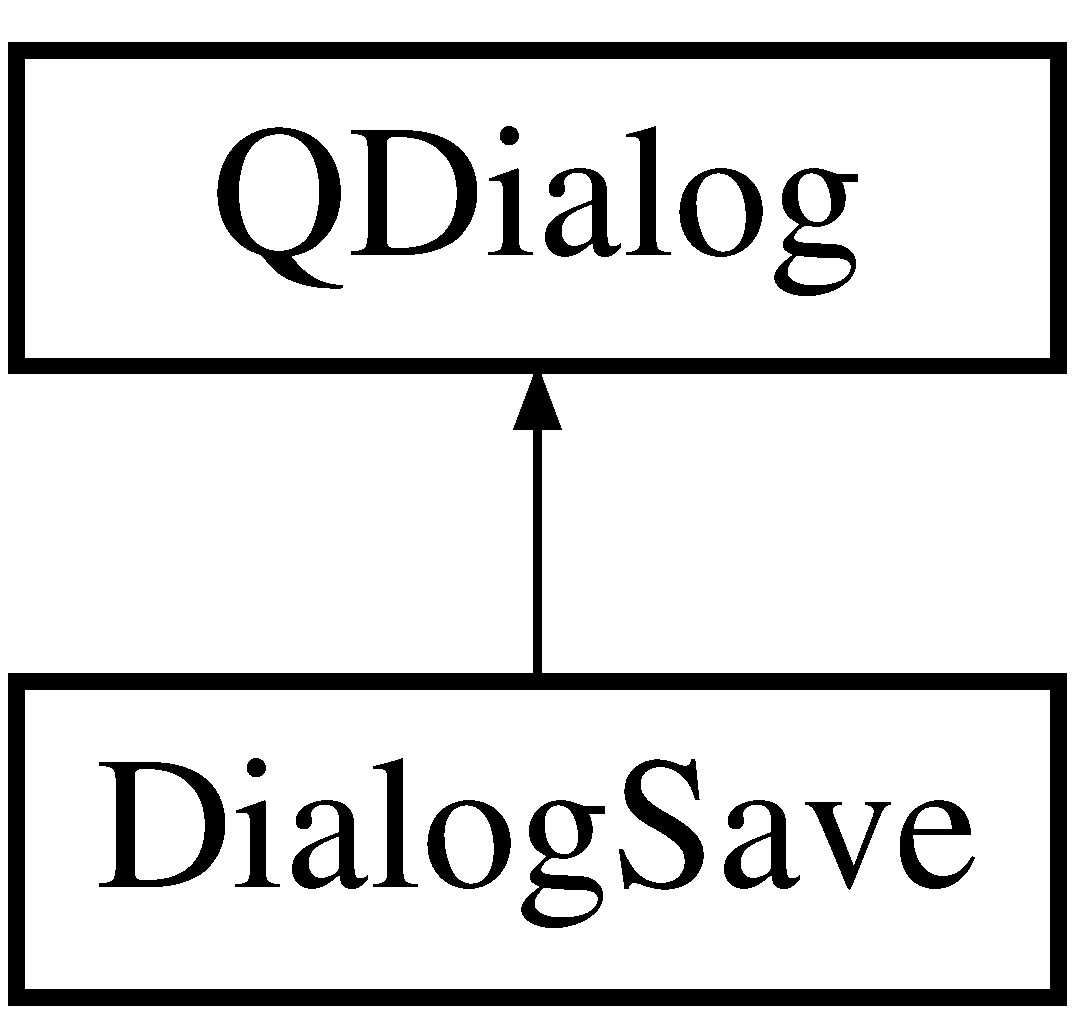
\includegraphics[height=2.000000cm]{classDialogSave}
\end{center}
\end{figure}
\subsection*{Public Slots}
\begin{DoxyCompactItemize}
\item 
\hypertarget{classDialogSave_a88af0b56e780534a18edabd9136ae9be}{void \hyperlink{classDialogSave_a88af0b56e780534a18edabd9136ae9be}{cancel\-Clicked} ()}\label{classDialogSave_a88af0b56e780534a18edabd9136ae9be}

\begin{DoxyCompactList}\small\item\em Closes the dialog and returns Rejected (this value is used by the exec function of the Q\-Dialog class) \end{DoxyCompactList}\item 
\hypertarget{classDialogSave_a3cbea9dd6b3efe8acf7149ac6b401724}{void \hyperlink{classDialogSave_a3cbea9dd6b3efe8acf7149ac6b401724}{quit\-Clicked} ()}\label{classDialogSave_a3cbea9dd6b3efe8acf7149ac6b401724}

\begin{DoxyCompactList}\small\item\em Closes the dialog and returns Accepted (this value is used by the exec function of the Q\-Dialog class) \end{DoxyCompactList}\end{DoxyCompactItemize}
\subsection*{Public Member Functions}
\begin{DoxyCompactItemize}
\item 
\hyperlink{classDialogSave_a6d5e21e7bf80d9f51020294eb35a5bff}{Dialog\-Save} (Q\-Widget $\ast$parent=0)
\begin{DoxyCompactList}\small\item\em \hyperlink{classDialogSave}{Dialog\-Save}. \end{DoxyCompactList}\end{DoxyCompactItemize}
\subsection*{Private Attributes}
\begin{DoxyCompactItemize}
\item 
\hypertarget{classDialogSave_a9a5fbd83fd9d699de19493bb6f00b18c}{Ui\-::\-Dialog\-Save $\ast$ {\bfseries ui}}\label{classDialogSave_a9a5fbd83fd9d699de19493bb6f00b18c}

\end{DoxyCompactItemize}


\subsection{Detailed Description}
The \hyperlink{classDialogSave}{Dialog\-Save} class manages the dialog shown when the user close the program but didn't save his file. 

\subsection{Constructor \& Destructor Documentation}
\hypertarget{classDialogSave_a6d5e21e7bf80d9f51020294eb35a5bff}{\index{Dialog\-Save@{Dialog\-Save}!Dialog\-Save@{Dialog\-Save}}
\index{Dialog\-Save@{Dialog\-Save}!DialogSave@{Dialog\-Save}}
\subsubsection[{Dialog\-Save}]{\setlength{\rightskip}{0pt plus 5cm}Dialog\-Save\-::\-Dialog\-Save (
\begin{DoxyParamCaption}
\item[{Q\-Widget $\ast$}]{parent = {\ttfamily 0}}
\end{DoxyParamCaption}
)\hspace{0.3cm}{\ttfamily [explicit]}}}\label{classDialogSave_a6d5e21e7bf80d9f51020294eb35a5bff}


\hyperlink{classDialogSave}{Dialog\-Save}. 


\begin{DoxyParams}{Parameters}
{\em parent} & \\
\hline
\end{DoxyParams}


The documentation for this class was generated from the following files\-:\begin{DoxyCompactItemize}
\item 
dialogsave.\-h\item 
dialogsave.\-cpp\end{DoxyCompactItemize}

\hypertarget{classMainWindow}{\section{Main\-Window Class Reference}
\label{classMainWindow}\index{Main\-Window@{Main\-Window}}
}


The \hyperlink{classMainWindow}{Main\-Window} class manages all the user interface.  




{\ttfamily \#include $<$mainwindow.\-h$>$}

Inheritance diagram for Main\-Window\-:\begin{figure}[H]
\begin{center}
\leavevmode
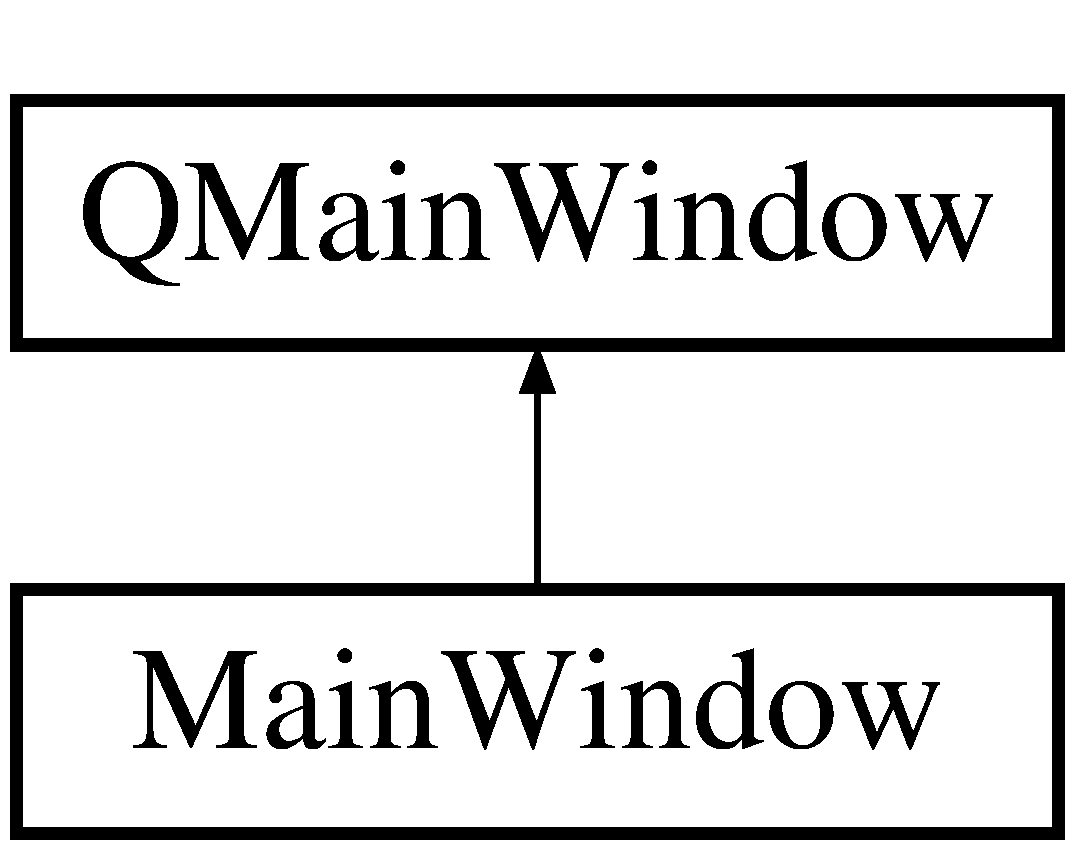
\includegraphics[height=2.000000cm]{classMainWindow}
\end{center}
\end{figure}
\subsection*{Public Slots}
\begin{DoxyCompactItemize}
\item 
\hypertarget{classMainWindow_a2ae51e1e864469c364b0f8ca9f001926}{void \hyperlink{classMainWindow_a2ae51e1e864469c364b0f8ca9f001926}{select\-File} ()}\label{classMainWindow_a2ae51e1e864469c364b0f8ca9f001926}

\begin{DoxyCompactList}\small\item\em Opens a dialog to select an X\-M\-L file and store the file slected in filename. \end{DoxyCompactList}\item 
void \hyperlink{classMainWindow_a91bb6afc2332387aabd2c56a060cea2e}{show\-Details} (Q\-Model\-Index index)
\begin{DoxyCompactList}\small\item\em Shows the list of editables elements for the node slected. Informations are shown in the right part of the window. \end{DoxyCompactList}\item 
\hypertarget{classMainWindow_a1725a0bf1d276bb1fbc57ef669d73208}{void \hyperlink{classMainWindow_a1725a0bf1d276bb1fbc57ef669d73208}{save\-File\-As} ()}\label{classMainWindow_a1725a0bf1d276bb1fbc57ef669d73208}

\begin{DoxyCompactList}\small\item\em Save the X\-M\-L file by replacing the file selected before. \end{DoxyCompactList}\item 
\hypertarget{classMainWindow_a464aaa4d378e7b2d814756a73d6e1ed6}{void \hyperlink{classMainWindow_a464aaa4d378e7b2d814756a73d6e1ed6}{save\-File} ()}\label{classMainWindow_a464aaa4d378e7b2d814756a73d6e1ed6}

\begin{DoxyCompactList}\small\item\em Opens a dialog to save the X\-M\-L file. \end{DoxyCompactList}\item 
\hypertarget{classMainWindow_a99d6bd9b5763e598eed579cd670d1298}{void \hyperlink{classMainWindow_a99d6bd9b5763e598eed579cd670d1298}{executable} ()}\label{classMainWindow_a99d6bd9b5763e598eed579cd670d1298}

\begin{DoxyCompactList}\small\item\em Opens a dialog to execute the O\-F\-E\-L\-I program. \end{DoxyCompactList}\item 
\hypertarget{classMainWindow_a961f84bb1d476d689527e925d06133f3}{void \hyperlink{classMainWindow_a961f84bb1d476d689527e925d06133f3}{add\-Param} ()}\label{classMainWindow_a961f84bb1d476d689527e925d06133f3}

\begin{DoxyCompactList}\small\item\em Updates the right part of the window and add two fields editables so the user can set the name and the value of a new attribute. \end{DoxyCompactList}\item 
\hypertarget{classMainWindow_a05d44eee1bef57891a25366b45e6c3b2}{void \hyperlink{classMainWindow_a05d44eee1bef57891a25366b45e6c3b2}{insert} ()}\label{classMainWindow_a05d44eee1bef57891a25366b45e6c3b2}

\begin{DoxyCompactList}\small\item\em Updates the tree (and the document) with the attributes modified or added by the user. \end{DoxyCompactList}\item 
\hypertarget{classMainWindow_add4a43152e4abb3e68c1541a2663e794}{void \hyperlink{classMainWindow_add4a43152e4abb3e68c1541a2663e794}{open\-Window\-Add\-Node} ()}\label{classMainWindow_add4a43152e4abb3e68c1541a2663e794}

\begin{DoxyCompactList}\small\item\em Opens a dialog to add a new node to the tree (and the document). \end{DoxyCompactList}\item 
\hypertarget{classMainWindow_aa0322653d852753a24a8974027c23f16}{void \hyperlink{classMainWindow_aa0322653d852753a24a8974027c23f16}{delete\-Selected\-Node} ()}\label{classMainWindow_aa0322653d852753a24a8974027c23f16}

\begin{DoxyCompactList}\small\item\em Deletes the selected node in the tree. \end{DoxyCompactList}\item 
\hypertarget{classMainWindow_a29fc99dbacbd3e451df12f6e6b01d7be}{void \hyperlink{classMainWindow_a29fc99dbacbd3e451df12f6e6b01d7be}{open\-Window\-Modify\-Node} ()}\label{classMainWindow_a29fc99dbacbd3e451df12f6e6b01d7be}

\begin{DoxyCompactList}\small\item\em Opens a dialog to modify the name of the selected node in the tree. \end{DoxyCompactList}\item 
void \hyperlink{classMainWindow_a7ead9d2b3de68f8ca35c3c4234c3316b}{delete\-Attribute} (Q\-String name\-Attribute)
\begin{DoxyCompactList}\small\item\em Delete a given attribute from a node. \end{DoxyCompactList}\item 
\hypertarget{classMainWindow_a85bdf02a928c14f368a54ab2fa92cc05}{void \hyperlink{classMainWindow_a85bdf02a928c14f368a54ab2fa92cc05}{clear\-Result} ()}\label{classMainWindow_a85bdf02a928c14f368a54ab2fa92cc05}

\begin{DoxyCompactList}\small\item\em Clears the text area where the results are shown. \end{DoxyCompactList}\item 
\hypertarget{classMainWindow_a3867c6fa0d0e97c5a9dcc7dd67ce528f}{void \hyperlink{classMainWindow_a3867c6fa0d0e97c5a9dcc7dd67ce528f}{copy\-To\-Clipboard} ()}\label{classMainWindow_a3867c6fa0d0e97c5a9dcc7dd67ce528f}

\begin{DoxyCompactList}\small\item\em Copies the contents of the text area to the clipboard. \end{DoxyCompactList}\item 
\hypertarget{classMainWindow_acb446340737c00f7970ee3cf56982679}{void \hyperlink{classMainWindow_acb446340737c00f7970ee3cf56982679}{open\-Recent} ()}\label{classMainWindow_acb446340737c00f7970ee3cf56982679}

\begin{DoxyCompactList}\small\item\em Opens the file on which the user clicked in the Recent files menu. \end{DoxyCompactList}\item 
\hypertarget{classMainWindow_a71a0deb7cce3c55d9bec6c1ce69c79b3}{void \hyperlink{classMainWindow_a71a0deb7cce3c55d9bec6c1ce69c79b3}{open\-Window\-Add\-Comment} ()}\label{classMainWindow_a71a0deb7cce3c55d9bec6c1ce69c79b3}

\begin{DoxyCompactList}\small\item\em Opens a dialog to add a new comment to the tree (and the document). \end{DoxyCompactList}\item 
\hypertarget{classMainWindow_a5636c1b5036dd958fc79e6507fc230f5}{void \hyperlink{classMainWindow_a5636c1b5036dd958fc79e6507fc230f5}{open\-Window\-About} ()}\label{classMainWindow_a5636c1b5036dd958fc79e6507fc230f5}

\begin{DoxyCompactList}\small\item\em Opens the dialog \char`\"{}about\char`\"{}. \end{DoxyCompactList}\end{DoxyCompactItemize}
\subsection*{Public Member Functions}
\begin{DoxyCompactItemize}
\item 
\hyperlink{classMainWindow_a8b244be8b7b7db1b08de2a2acb9409db}{Main\-Window} (Q\-Widget $\ast$parent=0)
\begin{DoxyCompactList}\small\item\em \hyperlink{classMainWindow}{Main\-Window}. \end{DoxyCompactList}\item 
\hypertarget{classMainWindow_ae98d00a93bc118200eeef9f9bba1dba7}{\hyperlink{classMainWindow_ae98d00a93bc118200eeef9f9bba1dba7}{$\sim$\-Main\-Window} ()}\label{classMainWindow_ae98d00a93bc118200eeef9f9bba1dba7}

\begin{DoxyCompactList}\small\item\em Destructor. \end{DoxyCompactList}\item 
void \hyperlink{classMainWindow_a39b737ba3023be40c3c8c03a264934b2}{open\-Datas} (Q\-String file\-Name)
\begin{DoxyCompactList}\small\item\em Opens the X\-M\-L file containing the datas needed to execute the O\-F\-E\-L\-I program and generate the tree associated. \end{DoxyCompactList}\item 
void \hyperlink{classMainWindow_acdc6db8778f0183a241c92dae9f138f0}{build\-Tree} (Q\-Dom\-Node doc, Q\-Standard\-Item\-Model $\ast$model, Q\-Standard\-Item $\ast$item, Q\-List$<$ int $>$ $\ast$nb\-Children, int child\-Number, Q\-List$<$ int $>$ $\ast$current\-Child, int current\-Level)
\begin{DoxyCompactList}\small\item\em Generates a Q\-Standard\-Item\-Model recursively from a Q\-Dom\-Document. This model can be used by a Tree\-View. \end{DoxyCompactList}\item 
void \hyperlink{classMainWindow_af90fffcac39eb4bc42810588408111c3}{get\-Tag\-Attributes} (Q\-List$<$ Q\-Standard\-Item $\ast$ $>$ $\ast$list, Q\-Dom\-Node doc)
\begin{DoxyCompactList}\small\item\em Gets the list of parameters from a specific tag. \end{DoxyCompactList}\item 
void \hyperlink{classMainWindow_a6ac713dd9f9fcee2b6d285bb0ae5d3d1}{add\-Column\-Model} (Q\-Standard\-Item\-Model $\ast$model, Q\-Dom\-Node doc)
\begin{DoxyCompactList}\small\item\em Adds an empty column to a Q\-Standard\-Item\-Model for each attribute contained in the given node. \end{DoxyCompactList}\item 
void \hyperlink{classMainWindow_ac886ea69c593b8906039e86a91697705}{height\-X\-M\-L} (Q\-Dom\-Node doc, int $\ast$height)
\begin{DoxyCompactList}\small\item\em Gets the maximum height in the Q\-Dom\-Document recursively. \end{DoxyCompactList}\item 
void \hyperlink{classMainWindow_ab1cd5d659de665dd74bb81eb8c8dbf5d}{nb\-Attributes\-Max} (Q\-Dom\-Node doc, int $\ast$nb\-Attributes)
\begin{DoxyCompactList}\small\item\em Gets the number of attributes maximum for a tag in the Q\-Dom\-Document recursively. \end{DoxyCompactList}\item 
void \hyperlink{classMainWindow_af34f3d4d5da8e2b7daf444e221809e0c}{get\-Tag\-List} (Q\-Dom\-Node doc, Q\-String\-List $\ast$tag\-List)
\begin{DoxyCompactList}\small\item\em Gets the list of tags in the Q\-Dom\-Document recursively. \end{DoxyCompactList}\item 
void \hyperlink{classMainWindow_a2988f42c5d8edc521b9368a61bd25677}{add\-Node} (Q\-String name\-Parent, Q\-String name\-Node, Q\-String text\-Node)
\begin{DoxyCompactList}\small\item\em Adds a node to the given parent. \end{DoxyCompactList}\item 
void \hyperlink{classMainWindow_a885f74bf6dbd209942899d3b2c50b5cd}{modify\-Node} (Q\-String node\-Selected, Q\-String new\-Name)
\begin{DoxyCompactList}\small\item\em Modifies the node currently selected in the tree. \end{DoxyCompactList}\item 
\hypertarget{classMainWindow_a832b124c66bb3cd641b7c6cea8b72a10}{void \hyperlink{classMainWindow_a832b124c66bb3cd641b7c6cea8b72a10}{clear\-Form\-Layout} ()}\label{classMainWindow_a832b124c66bb3cd641b7c6cea8b72a10}

\begin{DoxyCompactList}\small\item\em Removes all items from the form\-Layout. \end{DoxyCompactList}\item 
void \hyperlink{classMainWindow_aed133479c6ee8b81e351af9db464a9a7}{set\-Column\-Labels} (Q\-Standard\-Item\-Model $\ast$model)
\begin{DoxyCompactList}\small\item\em Modifies the names of the columns by an empty String. \end{DoxyCompactList}\item 
void \hyperlink{classMainWindow_a9c4f542263838b9ecd06eae839a42a34}{key\-Press\-Event} (Q\-Key\-Event $\ast$event)
\begin{DoxyCompactList}\small\item\em Specifies that the user can press the key return to insert new parameters if a text edit is focused. \end{DoxyCompactList}\item 
void \hyperlink{classMainWindow_a4e20a4a065fbb0e4d3532a45a0a91425}{close\-Event} (Q\-Close\-Event $\ast$event)
\begin{DoxyCompactList}\small\item\em Checks if the user saved his files, if not, shows a dialog to notify the user that he didn't save the file. Also saves the window geometry using Q\-Settings object. \end{DoxyCompactList}\item 
void \hyperlink{classMainWindow_a1ec3a16af19b96d0fd9cdf46cc892937}{set\-Settings} (Q\-String filename)
\begin{DoxyCompactList}\small\item\em For now saves the recent files opened by the user using Q\-Settings object. Can be used for save more settings. \end{DoxyCompactList}\item 
\hypertarget{classMainWindow_a596984787bd143548c5afac3cd582f1c}{void \hyperlink{classMainWindow_a596984787bd143548c5afac3cd582f1c}{update\-Menu\-Recent\-Files} ()}\label{classMainWindow_a596984787bd143548c5afac3cd582f1c}

\begin{DoxyCompactList}\small\item\em Updates the recent files menu. \end{DoxyCompactList}\item 
void \hyperlink{classMainWindow_a00e35cdb432258d1e72a880ec8dd29f0}{add\-Comment} (Q\-String name\-Parent, Q\-String comment, int selected\-Row)
\begin{DoxyCompactList}\small\item\em Adds a comment after the selected node. \end{DoxyCompactList}\item 
Q\-String \hyperlink{classMainWindow_a976df6253f65334c295d515405f49a2a}{get\-Settings\-File} ()
\begin{DoxyCompactList}\small\item\em Return the name of the settings file associated to the application. \end{DoxyCompactList}\item 
\hypertarget{classMainWindow_adb079736c866c781e030899cd83e82ca}{void \hyperlink{classMainWindow_adb079736c866c781e030899cd83e82ca}{update\-Tree} ()}\label{classMainWindow_adb079736c866c781e030899cd83e82ca}

\begin{DoxyCompactList}\small\item\em Updates the tree. This function needs to be called if the user adds a parameter, delete a node, add a node, modify a node... \end{DoxyCompactList}\end{DoxyCompactItemize}
\subsection*{Private Attributes}
\begin{DoxyCompactItemize}
\item 
\hypertarget{classMainWindow_a35466a70ed47252a0191168126a352a5}{Ui\-::\-Main\-Window $\ast$ {\bfseries ui}}\label{classMainWindow_a35466a70ed47252a0191168126a352a5}

\item 
\hypertarget{classMainWindow_a53fd1e1d3acbd985e622f97003c20e4e}{Q\-String {\bfseries filename}}\label{classMainWindow_a53fd1e1d3acbd985e622f97003c20e4e}

\item 
\hypertarget{classMainWindow_ab95d2b324604f48a9b4599a0d69c135a}{Q\-String {\bfseries node\-Name}}\label{classMainWindow_ab95d2b324604f48a9b4599a0d69c135a}

\item 
\hypertarget{classMainWindow_a03a6f597bea79dd8e2dd74f3d0195f48}{Q\-String {\bfseries root}}\label{classMainWindow_a03a6f597bea79dd8e2dd74f3d0195f48}

\item 
\hypertarget{classMainWindow_ab41d081fd36048cdc7f0f7b6d9af4855}{Q\-Model\-Index {\bfseries current\-Index}}\label{classMainWindow_ab41d081fd36048cdc7f0f7b6d9af4855}

\item 
\hypertarget{classMainWindow_acf359550b2cb8095eaa5a3a87fa7f9f3}{Q\-Dom\-Document $\ast$ {\bfseries current\-Document}}\label{classMainWindow_acf359550b2cb8095eaa5a3a87fa7f9f3}

\item 
\hypertarget{classMainWindow_aa1a1f8ce9c37a7ac70d21402759638b3}{Q\-Standard\-Item\-Model $\ast$ {\bfseries model}}\label{classMainWindow_aa1a1f8ce9c37a7ac70d21402759638b3}

\item 
\hypertarget{classMainWindow_a47316d915f71d763479d846c24d79268}{Q\-List$<$ Q\-Widget $\ast$ $>$ {\bfseries list}}\label{classMainWindow_a47316d915f71d763479d846c24d79268}

\item 
\hypertarget{classMainWindow_ad0a212146dfe4452f07c574773e9082c}{Q\-List$<$ Q\-Push\-Button $\ast$ $>$ {\bfseries list\-Button}}\label{classMainWindow_ad0a212146dfe4452f07c574773e9082c}

\item 
\hypertarget{classMainWindow_a91f8d3559167d4b4cb30d3956dbd1eac}{Q\-List$<$ Q\-Layout $\ast$ $>$ {\bfseries list\-Layout}}\label{classMainWindow_a91f8d3559167d4b4cb30d3956dbd1eac}

\item 
\hypertarget{classMainWindow_a7d0d2546e92bafb61163812b2254de83}{Q\-Signal\-Mapper $\ast$ {\bfseries signal\-Mapper}}\label{classMainWindow_a7d0d2546e92bafb61163812b2254de83}

\item 
\hypertarget{classMainWindow_a2d4d28e971f741bdc7d6d0368ca4a503}{Q\-Clipboard $\ast$ {\bfseries clipboard}}\label{classMainWindow_a2d4d28e971f741bdc7d6d0368ca4a503}

\item 
\hypertarget{classMainWindow_a0bc74c3bb5204ac704e3b49551ba7e7e}{Q\-String\-List {\bfseries list\-Expanded}}\label{classMainWindow_a0bc74c3bb5204ac704e3b49551ba7e7e}

\item 
\hypertarget{classMainWindow_a3c243482183e39e41952044b97054d33}{bool {\bfseries file\-Saved}}\label{classMainWindow_a3c243482183e39e41952044b97054d33}

\item 
\hypertarget{classMainWindow_a87b5b9562fe91ee19249f5a0d7617ce0}{Q\-Settings {\bfseries settings}}\label{classMainWindow_a87b5b9562fe91ee19249f5a0d7617ce0}

\item 
\hypertarget{classMainWindow_a33c4f37d91dfcb191075b1f9de98a407}{Q\-Menu $\ast$ {\bfseries menu\-Recent\-Files}}\label{classMainWindow_a33c4f37d91dfcb191075b1f9de98a407}

\item 
\hypertarget{classMainWindow_ab46d72b4942ac8270ea113df0c5d12e9}{bool {\bfseries model\-Is\-Set}}\label{classMainWindow_ab46d72b4942ac8270ea113df0c5d12e9}

\item 
\hypertarget{classMainWindow_a16d41d6fadc8befa5afa12460580334a}{Q\-Grid\-Layout $\ast$ {\bfseries grid\-Layout}}\label{classMainWindow_a16d41d6fadc8befa5afa12460580334a}

\item 
\hypertarget{classMainWindow_a90866e624993aa14910a2c66eb2272d4}{Q\-Tree\-View $\ast$ {\bfseries tree\-View}}\label{classMainWindow_a90866e624993aa14910a2c66eb2272d4}

\item 
\hypertarget{classMainWindow_a9d53657ebe6ee2f3051520304b495f52}{Q\-Text\-Edit $\ast$ {\bfseries text\-Result}}\label{classMainWindow_a9d53657ebe6ee2f3051520304b495f52}

\item 
\hypertarget{classMainWindow_a3a8f2713f53485c32f3e4d08b0740e09}{Q\-Push\-Button $\ast$ {\bfseries button\-Save}}\label{classMainWindow_a3a8f2713f53485c32f3e4d08b0740e09}

\item 
\hypertarget{classMainWindow_ab0826d7f35af5835844ab2028080e102}{Q\-Push\-Button $\ast$ {\bfseries button\-Exec}}\label{classMainWindow_ab0826d7f35af5835844ab2028080e102}

\item 
\hypertarget{classMainWindow_ae0a75bbbae685e3a6c36e24571e4ef56}{Q\-Push\-Button $\ast$ {\bfseries button\-Add\-Param}}\label{classMainWindow_ae0a75bbbae685e3a6c36e24571e4ef56}

\item 
\hypertarget{classMainWindow_ad7b85d9b1021e56de3dd061541d0a9f2}{Q\-Push\-Button $\ast$ {\bfseries button\-Insert}}\label{classMainWindow_ad7b85d9b1021e56de3dd061541d0a9f2}

\item 
\hypertarget{classMainWindow_a1cff650d7154e197cac5c2c6928cc404}{Q\-Form\-Layout $\ast$ {\bfseries form\-Layout}}\label{classMainWindow_a1cff650d7154e197cac5c2c6928cc404}

\item 
\hypertarget{classMainWindow_a89e281849b9cf7d03662402c6bc6012c}{Q\-Label $\ast$ {\bfseries label}}\label{classMainWindow_a89e281849b9cf7d03662402c6bc6012c}

\item 
\hypertarget{classMainWindow_aeaa79ec646e5180f0933332eee711d41}{Q\-Push\-Button $\ast$ {\bfseries button\-Clear}}\label{classMainWindow_aeaa79ec646e5180f0933332eee711d41}

\item 
\hypertarget{classMainWindow_a82b8cf27f799696be731caf0850bd4be}{Q\-Push\-Button $\ast$ {\bfseries button\-Copy}}\label{classMainWindow_a82b8cf27f799696be731caf0850bd4be}

\item 
\hypertarget{classMainWindow_afd6c41d06a82259f974595df3970abc5}{Q\-Scroll\-Area $\ast$ {\bfseries scroll\-Container}}\label{classMainWindow_afd6c41d06a82259f974595df3970abc5}

\item 
\hypertarget{classMainWindow_ae35513d881514a697aadf7437df70d2b}{Q\-Widget $\ast$ {\bfseries scrollable\-Widget}}\label{classMainWindow_ae35513d881514a697aadf7437df70d2b}

\item 
\hypertarget{classMainWindow_a392fb761a37795ee8081438c8c3493dd}{Q\-Splitter $\ast$ {\bfseries splitter}}\label{classMainWindow_a392fb761a37795ee8081438c8c3493dd}

\end{DoxyCompactItemize}


\subsection{Detailed Description}
The \hyperlink{classMainWindow}{Main\-Window} class manages all the user interface. 

\subsection{Constructor \& Destructor Documentation}
\hypertarget{classMainWindow_a8b244be8b7b7db1b08de2a2acb9409db}{\index{Main\-Window@{Main\-Window}!Main\-Window@{Main\-Window}}
\index{Main\-Window@{Main\-Window}!MainWindow@{Main\-Window}}
\subsubsection[{Main\-Window}]{\setlength{\rightskip}{0pt plus 5cm}Main\-Window\-::\-Main\-Window (
\begin{DoxyParamCaption}
\item[{Q\-Widget $\ast$}]{parent = {\ttfamily 0}}
\end{DoxyParamCaption}
)\hspace{0.3cm}{\ttfamily [explicit]}}}\label{classMainWindow_a8b244be8b7b7db1b08de2a2acb9409db}


\hyperlink{classMainWindow}{Main\-Window}. 


\begin{DoxyParams}{Parameters}
{\em parent} & \\
\hline
\end{DoxyParams}


\subsection{Member Function Documentation}
\hypertarget{classMainWindow_a6ac713dd9f9fcee2b6d285bb0ae5d3d1}{\index{Main\-Window@{Main\-Window}!add\-Column\-Model@{add\-Column\-Model}}
\index{add\-Column\-Model@{add\-Column\-Model}!MainWindow@{Main\-Window}}
\subsubsection[{add\-Column\-Model}]{\setlength{\rightskip}{0pt plus 5cm}void Main\-Window\-::add\-Column\-Model (
\begin{DoxyParamCaption}
\item[{Q\-Standard\-Item\-Model $\ast$}]{model, }
\item[{Q\-Dom\-Node}]{doc}
\end{DoxyParamCaption}
)}}\label{classMainWindow_a6ac713dd9f9fcee2b6d285bb0ae5d3d1}


Adds an empty column to a Q\-Standard\-Item\-Model for each attribute contained in the given node. 


\begin{DoxyParams}{Parameters}
{\em model} & The model on which you want to add a column \\
\hline
{\em doc} & A node \\
\hline
\end{DoxyParams}
\hypertarget{classMainWindow_a00e35cdb432258d1e72a880ec8dd29f0}{\index{Main\-Window@{Main\-Window}!add\-Comment@{add\-Comment}}
\index{add\-Comment@{add\-Comment}!MainWindow@{Main\-Window}}
\subsubsection[{add\-Comment}]{\setlength{\rightskip}{0pt plus 5cm}void Main\-Window\-::add\-Comment (
\begin{DoxyParamCaption}
\item[{Q\-String}]{name\-Parent, }
\item[{Q\-String}]{comment, }
\item[{int}]{selected\-Row}
\end{DoxyParamCaption}
)}}\label{classMainWindow_a00e35cdb432258d1e72a880ec8dd29f0}


Adds a comment after the selected node. 


\begin{DoxyParams}{Parameters}
{\em name\-Parent} & The name of the parent of the node selected \\
\hline
{\em comment} & The comment to add \\
\hline
{\em selected\-Row} & The row number of the slected node \\
\hline
\end{DoxyParams}
\hypertarget{classMainWindow_a2988f42c5d8edc521b9368a61bd25677}{\index{Main\-Window@{Main\-Window}!add\-Node@{add\-Node}}
\index{add\-Node@{add\-Node}!MainWindow@{Main\-Window}}
\subsubsection[{add\-Node}]{\setlength{\rightskip}{0pt plus 5cm}void Main\-Window\-::add\-Node (
\begin{DoxyParamCaption}
\item[{Q\-String}]{name\-Parent, }
\item[{Q\-String}]{name\-Node, }
\item[{Q\-String}]{text\-Node}
\end{DoxyParamCaption}
)}}\label{classMainWindow_a2988f42c5d8edc521b9368a61bd25677}


Adds a node to the given parent. 


\begin{DoxyParams}{Parameters}
{\em name\-Parent} & The tag name of the parent \\
\hline
{\em name\-Node} & The tag name of the node to add \\
\hline
{\em text\-Node} & The text to insert in the node \\
\hline
\end{DoxyParams}
\hypertarget{classMainWindow_acdc6db8778f0183a241c92dae9f138f0}{\index{Main\-Window@{Main\-Window}!build\-Tree@{build\-Tree}}
\index{build\-Tree@{build\-Tree}!MainWindow@{Main\-Window}}
\subsubsection[{build\-Tree}]{\setlength{\rightskip}{0pt plus 5cm}void Main\-Window\-::build\-Tree (
\begin{DoxyParamCaption}
\item[{Q\-Dom\-Node}]{doc, }
\item[{Q\-Standard\-Item\-Model $\ast$}]{model, }
\item[{Q\-Standard\-Item $\ast$}]{item, }
\item[{Q\-List$<$ int $>$ $\ast$}]{nb\-Children, }
\item[{int}]{child\-Number, }
\item[{Q\-List$<$ int $>$ $\ast$}]{current\-Child, }
\item[{int}]{current\-Level}
\end{DoxyParamCaption}
)}}\label{classMainWindow_acdc6db8778f0183a241c92dae9f138f0}


Generates a Q\-Standard\-Item\-Model recursively from a Q\-Dom\-Document. This model can be used by a Tree\-View. 


\begin{DoxyParams}{Parameters}
{\em doc} & A Q\-Dom\-Node containing the root of your Q\-Dom\-Document \\
\hline
{\em model} & An empty Q\-Standard\-Item\-Model \\
\hline
{\em item} & A Q\-Standard\-Item containing a Q\-String which is the tag name of the root \\
\hline
{\em nb\-Children} & A list containing only zeros. Its length must be equals to the maximum height of the Q\-Dom\-Document \\
\hline
{\em child\-Number} & Must be 0 for the first call. \\
\hline
{\em current\-Child} & A list containing only zeros. Its length must be equals to the maximum height of the Q\-Dom\-Document \\
\hline
{\em current\-Level} & Must be -\/1 for the first call. \\
\hline
\end{DoxyParams}
\hypertarget{classMainWindow_a4e20a4a065fbb0e4d3532a45a0a91425}{\index{Main\-Window@{Main\-Window}!close\-Event@{close\-Event}}
\index{close\-Event@{close\-Event}!MainWindow@{Main\-Window}}
\subsubsection[{close\-Event}]{\setlength{\rightskip}{0pt plus 5cm}void Main\-Window\-::close\-Event (
\begin{DoxyParamCaption}
\item[{Q\-Close\-Event $\ast$}]{event}
\end{DoxyParamCaption}
)}}\label{classMainWindow_a4e20a4a065fbb0e4d3532a45a0a91425}


Checks if the user saved his files, if not, shows a dialog to notify the user that he didn't save the file. Also saves the window geometry using Q\-Settings object. 


\begin{DoxyParams}{Parameters}
{\em event} & \\
\hline
\end{DoxyParams}
\hypertarget{classMainWindow_a7ead9d2b3de68f8ca35c3c4234c3316b}{\index{Main\-Window@{Main\-Window}!delete\-Attribute@{delete\-Attribute}}
\index{delete\-Attribute@{delete\-Attribute}!MainWindow@{Main\-Window}}
\subsubsection[{delete\-Attribute}]{\setlength{\rightskip}{0pt plus 5cm}void Main\-Window\-::delete\-Attribute (
\begin{DoxyParamCaption}
\item[{Q\-String}]{name\-Attribute}
\end{DoxyParamCaption}
)\hspace{0.3cm}{\ttfamily [slot]}}}\label{classMainWindow_a7ead9d2b3de68f8ca35c3c4234c3316b}


Delete a given attribute from a node. 


\begin{DoxyParams}{Parameters}
{\em name\-Attribute} & The name of the attribute to delete. \\
\hline
\end{DoxyParams}
\hypertarget{classMainWindow_a976df6253f65334c295d515405f49a2a}{\index{Main\-Window@{Main\-Window}!get\-Settings\-File@{get\-Settings\-File}}
\index{get\-Settings\-File@{get\-Settings\-File}!MainWindow@{Main\-Window}}
\subsubsection[{get\-Settings\-File}]{\setlength{\rightskip}{0pt plus 5cm}Q\-String Main\-Window\-::get\-Settings\-File (
\begin{DoxyParamCaption}
{}
\end{DoxyParamCaption}
)}}\label{classMainWindow_a976df6253f65334c295d515405f49a2a}


Return the name of the settings file associated to the application. 

\begin{DoxyReturn}{Returns}

\end{DoxyReturn}
\hypertarget{classMainWindow_af90fffcac39eb4bc42810588408111c3}{\index{Main\-Window@{Main\-Window}!get\-Tag\-Attributes@{get\-Tag\-Attributes}}
\index{get\-Tag\-Attributes@{get\-Tag\-Attributes}!MainWindow@{Main\-Window}}
\subsubsection[{get\-Tag\-Attributes}]{\setlength{\rightskip}{0pt plus 5cm}void Main\-Window\-::get\-Tag\-Attributes (
\begin{DoxyParamCaption}
\item[{Q\-List$<$ Q\-Standard\-Item $\ast$ $>$ $\ast$}]{list, }
\item[{Q\-Dom\-Node}]{doc}
\end{DoxyParamCaption}
)}}\label{classMainWindow_af90fffcac39eb4bc42810588408111c3}


Gets the list of parameters from a specific tag. 


\begin{DoxyParams}{Parameters}
{\em list} & Contains the outpout \\
\hline
{\em doc} & The node from which you want to get the list of attributes \\
\hline
\end{DoxyParams}
\hypertarget{classMainWindow_af34f3d4d5da8e2b7daf444e221809e0c}{\index{Main\-Window@{Main\-Window}!get\-Tag\-List@{get\-Tag\-List}}
\index{get\-Tag\-List@{get\-Tag\-List}!MainWindow@{Main\-Window}}
\subsubsection[{get\-Tag\-List}]{\setlength{\rightskip}{0pt plus 5cm}void Main\-Window\-::get\-Tag\-List (
\begin{DoxyParamCaption}
\item[{Q\-Dom\-Node}]{doc, }
\item[{Q\-String\-List $\ast$}]{tag\-List}
\end{DoxyParamCaption}
)}}\label{classMainWindow_af34f3d4d5da8e2b7daf444e221809e0c}


Gets the list of tags in the Q\-Dom\-Document recursively. 


\begin{DoxyParams}{Parameters}
{\em doc} & The root of the document \\
\hline
{\em tag\-List} & An empty Q\-String\-List. Contains the output \\
\hline
\end{DoxyParams}
\hypertarget{classMainWindow_ac886ea69c593b8906039e86a91697705}{\index{Main\-Window@{Main\-Window}!height\-X\-M\-L@{height\-X\-M\-L}}
\index{height\-X\-M\-L@{height\-X\-M\-L}!MainWindow@{Main\-Window}}
\subsubsection[{height\-X\-M\-L}]{\setlength{\rightskip}{0pt plus 5cm}void Main\-Window\-::height\-X\-M\-L (
\begin{DoxyParamCaption}
\item[{Q\-Dom\-Node}]{doc, }
\item[{int $\ast$}]{height}
\end{DoxyParamCaption}
)}}\label{classMainWindow_ac886ea69c593b8906039e86a91697705}


Gets the maximum height in the Q\-Dom\-Document recursively. 


\begin{DoxyParams}{Parameters}
{\em doc} & The root of the document \\
\hline
{\em height} & Must be 0 for the first call. Contains the output \\
\hline
\end{DoxyParams}
\hypertarget{classMainWindow_a9c4f542263838b9ecd06eae839a42a34}{\index{Main\-Window@{Main\-Window}!key\-Press\-Event@{key\-Press\-Event}}
\index{key\-Press\-Event@{key\-Press\-Event}!MainWindow@{Main\-Window}}
\subsubsection[{key\-Press\-Event}]{\setlength{\rightskip}{0pt plus 5cm}void Main\-Window\-::key\-Press\-Event (
\begin{DoxyParamCaption}
\item[{Q\-Key\-Event $\ast$}]{event}
\end{DoxyParamCaption}
)}}\label{classMainWindow_a9c4f542263838b9ecd06eae839a42a34}


Specifies that the user can press the key return to insert new parameters if a text edit is focused. 


\begin{DoxyParams}{Parameters}
{\em event} & \\
\hline
\end{DoxyParams}
\hypertarget{classMainWindow_a885f74bf6dbd209942899d3b2c50b5cd}{\index{Main\-Window@{Main\-Window}!modify\-Node@{modify\-Node}}
\index{modify\-Node@{modify\-Node}!MainWindow@{Main\-Window}}
\subsubsection[{modify\-Node}]{\setlength{\rightskip}{0pt plus 5cm}void Main\-Window\-::modify\-Node (
\begin{DoxyParamCaption}
\item[{Q\-String}]{node\-Selected, }
\item[{Q\-String}]{new\-Name}
\end{DoxyParamCaption}
)}}\label{classMainWindow_a885f74bf6dbd209942899d3b2c50b5cd}


Modifies the node currently selected in the tree. 


\begin{DoxyParams}{Parameters}
{\em node\-Selected} & The name of the node selected \\
\hline
{\em new\-Name} & The new name of the node \\
\hline
\end{DoxyParams}
\hypertarget{classMainWindow_ab1cd5d659de665dd74bb81eb8c8dbf5d}{\index{Main\-Window@{Main\-Window}!nb\-Attributes\-Max@{nb\-Attributes\-Max}}
\index{nb\-Attributes\-Max@{nb\-Attributes\-Max}!MainWindow@{Main\-Window}}
\subsubsection[{nb\-Attributes\-Max}]{\setlength{\rightskip}{0pt plus 5cm}void Main\-Window\-::nb\-Attributes\-Max (
\begin{DoxyParamCaption}
\item[{Q\-Dom\-Node}]{doc, }
\item[{int $\ast$}]{nb\-Attributes}
\end{DoxyParamCaption}
)}}\label{classMainWindow_ab1cd5d659de665dd74bb81eb8c8dbf5d}


Gets the number of attributes maximum for a tag in the Q\-Dom\-Document recursively. 


\begin{DoxyParams}{Parameters}
{\em doc} & The root of the document \\
\hline
{\em nb\-Attributes} & Must be 0 for the first call. Contains the output \\
\hline
\end{DoxyParams}
\hypertarget{classMainWindow_a39b737ba3023be40c3c8c03a264934b2}{\index{Main\-Window@{Main\-Window}!open\-Datas@{open\-Datas}}
\index{open\-Datas@{open\-Datas}!MainWindow@{Main\-Window}}
\subsubsection[{open\-Datas}]{\setlength{\rightskip}{0pt plus 5cm}void Main\-Window\-::open\-Datas (
\begin{DoxyParamCaption}
\item[{Q\-String}]{file\-Name}
\end{DoxyParamCaption}
)}}\label{classMainWindow_a39b737ba3023be40c3c8c03a264934b2}


Opens the X\-M\-L file containing the datas needed to execute the O\-F\-E\-L\-I program and generate the tree associated. 


\begin{DoxyParams}{Parameters}
{\em file\-Name} & A Q\-String containing the path to the X\-M\-L file \\
\hline
\end{DoxyParams}
\hypertarget{classMainWindow_aed133479c6ee8b81e351af9db464a9a7}{\index{Main\-Window@{Main\-Window}!set\-Column\-Labels@{set\-Column\-Labels}}
\index{set\-Column\-Labels@{set\-Column\-Labels}!MainWindow@{Main\-Window}}
\subsubsection[{set\-Column\-Labels}]{\setlength{\rightskip}{0pt plus 5cm}void Main\-Window\-::set\-Column\-Labels (
\begin{DoxyParamCaption}
\item[{Q\-Standard\-Item\-Model $\ast$}]{model}
\end{DoxyParamCaption}
)}}\label{classMainWindow_aed133479c6ee8b81e351af9db464a9a7}


Modifies the names of the columns by an empty String. 


\begin{DoxyParams}{Parameters}
{\em model} & \\
\hline
\end{DoxyParams}
\hypertarget{classMainWindow_a1ec3a16af19b96d0fd9cdf46cc892937}{\index{Main\-Window@{Main\-Window}!set\-Settings@{set\-Settings}}
\index{set\-Settings@{set\-Settings}!MainWindow@{Main\-Window}}
\subsubsection[{set\-Settings}]{\setlength{\rightskip}{0pt plus 5cm}void Main\-Window\-::set\-Settings (
\begin{DoxyParamCaption}
\item[{Q\-String}]{filename}
\end{DoxyParamCaption}
)}}\label{classMainWindow_a1ec3a16af19b96d0fd9cdf46cc892937}


For now saves the recent files opened by the user using Q\-Settings object. Can be used for save more settings. 


\begin{DoxyParams}{Parameters}
{\em filename} & \\
\hline
\end{DoxyParams}
\hypertarget{classMainWindow_a91bb6afc2332387aabd2c56a060cea2e}{\index{Main\-Window@{Main\-Window}!show\-Details@{show\-Details}}
\index{show\-Details@{show\-Details}!MainWindow@{Main\-Window}}
\subsubsection[{show\-Details}]{\setlength{\rightskip}{0pt plus 5cm}void Main\-Window\-::show\-Details (
\begin{DoxyParamCaption}
\item[{Q\-Model\-Index}]{index}
\end{DoxyParamCaption}
)\hspace{0.3cm}{\ttfamily [slot]}}}\label{classMainWindow_a91bb6afc2332387aabd2c56a060cea2e}


Shows the list of editables elements for the node slected. Informations are shown in the right part of the window. 


\begin{DoxyParams}{Parameters}
{\em index} & Index of the node selected in the tree \\
\hline
\end{DoxyParams}


The documentation for this class was generated from the following files\-:\begin{DoxyCompactItemize}
\item 
mainwindow.\-h\item 
mainwindow.\-cpp\end{DoxyCompactItemize}

%--- End generated contents ---

% Index
\newpage
\phantomsection
\addcontentsline{toc}{chapter}{Index}
\printindex

\end{document}
